% podobne prace?

\chapter{Experiment}
Experimentom v našej práci je meranie hĺbky pamäte a vyhodnotenie vplyvu rôznych
hyper parametrov a typov kontextov na hĺbku pamäte sietí. 
Cieľom nášho experimentu je aj nájdenie 
optimálnej kombinácie parametrov pre všetky typy porovnávaných sietí a porovnanie sietí.

\section{Výber trénovacích množín pre experiment}
Trénovacie množiny nie sú vybrané náhodne, ale snažili sme sa ich vytvoriť
takým spôsobom aby sme na nich vedeli otestovať rôzne vlastnosti rekurentných sietí.

Prvý dataset pozostáva z náhodne generovanej sekvencie znakov "abcd" dlhej 1000 znakov.
Druhý dataset pozostáva z reberovým stringom, ktoré sú generované reberovým automatom.

Tento bude dôležitý najmä pri trénovaní a testovaní SRN, kde by sme mohli dostať zaujímavé výsledky.

Tretí dataset je úryvok textu z nejakého korpusu angli ckého textu. 
Keďže ide o reálny zmysluplný text, nie je to úplne náhodná postupnosť znakov, ale obsahuje určité vzory a opakovania, ktoré by siete mohli vedieť zachytiť
vo svojej vnútorenej reprezentácii.
Tento dataset slúži iba ako "benchmark", ktorý nám povie, či sa sieť dokáže naučiť aj na reálnych textoch.

\section{Hľadanie optimálnych parametrov sietí}
Na to aby sme mohli porovnať hĺbku pamäte rôznych typov sietí museli sme nájsť kombináciu parametrov
pri ktorých daný typ siete dosahuje najlepšie výsledky. 
Pri trénovaní samoorganizujúcich sa máp môžeme meniť a optimalizovať veľké množstvo parametrov. 

Všeobecne pri trénovaní SOM je dôležité 
nastaviť správnu veľkosť okolia, ktorá by mala počas trénovania postupne klesať.
Veľkosť okolie neurónu v určitom kroku trénovania určuje excitačná funkcia, ktorá používa
spojité gausovské okolie.
\begin{equation}
    N(i^{*}, i) = \exp^{- \frac{d^{2}_{E}(i^{*}, i)}{\lambda^{2}(t)}}
\end{equation}
Dôležitý je parameter $\lambda$, ktorým znižujem veľkosť okolia postupne v jednotlivých epochách.
Najlepšie výsledky (najnižšie hodnoty kvantizačnej chyby) sme dosiahli pri použití nasledujúceho vzťahu pre výpočet hodnoty tohto parametra
v jednotlivých epochách:
\begin{equation}
    \lambda{(t)} = \lambda_{i} \cdot (\lambda_{f} /\ \lambda_{i})^{t /\ t_{max}}
\end{equation}
Kde $\lambda_{f}$ je konštanta, ktorá určuje rýchlosť klesania. 
$\lambda_{i}$ je polovica maximálnej vzdialenosti dvoch neurónov v mape, resp. 
vzdialenosť dvoch neurónov na koncoch diagonály.
$t$ je číslo aktuálnej epochy trénovania. Parametrer $t_{max}$ je počet 
epôch trénovania.


\subsection{RecSOM parametre}
Pri RecSOM kontext tvorí vektor excitácii neurónov z predchádzajúceho kroku.
Excitácia neurónu $y$ je určená vzťahom a neobsahuje žiadny meniteľný parameter. 
$d_{i}$ je súčet vzdialenosti vstupného vektora od váhového vektora a kontextového vektora od 
kontextového vektora. So zmenšujúcou sa vzdialenosťou excitácia neurónu rastie exponenciálne, čo 
znamená, že víťaz bude mať najvyššiu excitáciu.
\begin{equation}
    y_{i} = \exp{(-d_{i})}
\end{equation}

Môžeme meniť parameter $\alpha$, ktorý sa používa pri samotnej výpočte vzdialenosti
vstupu od váhového vektora a kontextu od vkontextového vektora. Tento parameter určuje váhu aktuálneho vstupu a váhu kontextu
vo výslednej vzdialenosti.
\begin{equation}
	d_i = (1 - \alpha) \cdot ||x(t) - w_i||^{2} + \alpha \cdot ||y(t-1) - c_i||^{2} \quad c \in R^{N}
\end{equation}
V našich experimentoch sme testovali všetky hodnoty parametra $\alpha$ z uzavretého intervalu
$<0, 1>$ s krokom $0.01$ (100 experimentov).

% tabulka, konkrtetne pouzite parametre

Výsledky: \\

% výsledky experimentu
\subsection{Activity RecSOM parametre}
Pri modifikovanej verzii RecSOM v ktorej počítame aktivitu neurónov
odlišným spôsobom máme tiež $\beta$ parameter. 
Na výpočet aktivity neurónu používame gaussovskú funkciu, ktorej priebeh ovplyvňujeme
pomocou $\beta$ parametra. To znamená, už to nie je exponenciálna funkcia, ale má odlišný priebeh, 
čo ovplyvňuje výsledné hodnoty aktivácii jednotlivých neurónov. Navyše výslednú hodnotu normalizujeme na
hodnoty z intervalu $<0, 1>$.
\begin{equation}
    \exp^{-\beta \cdot d^2}
\end{equation}

V experimente sme skúšali všetky kombinácie parametrov $\alpha$ a $\beta$.


\subsection{MSOM parametre}
Pri mSOM máme okrem $\alpha$ parametra aj $\beta$ parameter, ktorý určuje váhu
váhového vektora víťaza z predchádzajúceho kroku $w_{i^{*}}$ a váhu kontextu
z predchádzajúceho kroku $y_{i^{*}}$.
V našom experimente skúšame všetky kombinácie $\alpha$ a $\beta$ parametrov.
Hodnoty pre oba parametre sú z uzavretého intervalu $<0, 1>$ s krokom $0.1$ (100 experimentov).


\subsection{Decaying MSOM parametre}
Pri modifikovanej verzii mSOM máme, podobne ako pri mSOM, $\beta$ parameter, ktorý vo vzťahu 
pre výpočet kontextu určuje váhy jednotlivých minulých vstupov. Čím vyššia je hodnota $\beta$
parametra tým vyššiu váhu majú jednotlivé minulé vstupy.
Opäť skúšame všetky kombinácie $\alpha$ a $\beta$ parametrov.
Hodnoty pre oba parametre sú, podobne ako pri mSOM, z uzavretého intervalu $<0, 1>$ s krokom $0.1$

% vysledky



Experimentami sme zistili, že na hĺbku pamäte siete majú vplyv iba niektoré z nich. 
Najdôležitejšie parameters, ktoré vplývajú na hĺbku pamäte neurónovej siete sú parameters $\alpha$ a $\beta$
vo vzťahu pre výpočet vzdialenosti vstupného vektora od určitého neurónu v siete (čiže od jeho váhového a kontextového vektora).
% TODO pridat rovnicu na ilustraciu
Tieto dva parameters určujú pomer dôležitosti aktuálneho vstupu a dôležitosť kontextu, pri výpočte vzdialenosti (kvantizačnej chyby).

Experiment prebiehal nasledujúcim spôsobom:
\begin{itemize}
    \item Vybrali sme vhodnú trénovaciu sekvenciu, počet epôch trénovania a dostatočnú veľkosť pamäťového okna
    \item Spustili sme trénovanie na všetkých kombináciach týchto dvoch parametrov s krokom 0.1
    \item Hodnoty pamäťovej hĺbky sme ukladali do súboru
    \item Na záver sme vykreslili heatmapu, ktorá znázorňuje aká bola pamäťová hĺbka pre rôzne kombinácie parametrov.
\end{itemize}

% TODO vyber rychlosti ucenia (konstantna / postupne zmensujuca?)

Počet epôch sme určili na základe kvantizačnej chyby.
Počet epôch sme postupne zvyšovali a keď kvantizačná chyba prestala signifikantne klesať, resp. dosiahla 
svoje minimum zastavali sme ho na tejto hodnote a ďalej nezvyšovali. SOM sa dokážu relatívne rýchlo učiť a 
teda počet epôch nemusí byť vysoký, čo je veľkou výhodou pri experimentovaní, kedže trénovanie netrvá príliš dlhú dobu
a tým pádom sme mohli vyskúšať viac kombinácii a modifikácii.

Dostatočnú veľkosť pamäťového okna sme určili podobne ako počet epôch. Parameter sme postupne zvyšovali
a zastavili na hodnote, keď pamäťová hĺbka siete prestala stúpať, čiže veľkosť pamäťového okna už
neovplyvňovala hĺbku pamäte a ďalšie zvyšovanie parametra nemalo zmysel. 

Na základe tohto sme zistili, že pre každý typ siete sú ideálne hodnoty týchto parametrov odlišné.


\section{Vyhodnotenie rôznych kombinácii alpha a beta parametrov}

The table \ref{table:1} is an example of referenced \LaTeX elements.
 
\begin{table}[h!]
\centering
\begin{tabular}{|c|c|} 
 \hline
 Parameter & Hodnota \\ 
 \hline\hline
 1 & 6  \\ 
 \hline
 2 & 7   \\
 \hline
 3 & 545  \\
 \hline
 4 & 545  \\
 \hline
 5 & 88 \\  
 \hline
\end{tabular}
\caption{Parametre RecSOM siete}
\label{table:1}
\end{table}


\begin{figure}[H]
    \centering
    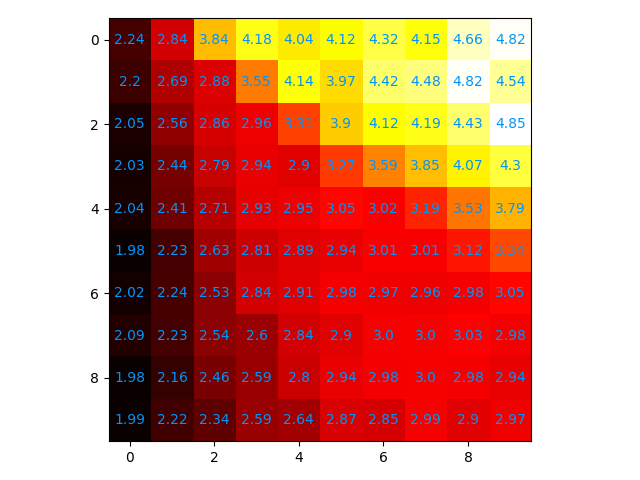
\includegraphics[width=8cm]{assets/recsom_abcd}
    \caption{Rec SOM results}
\end{figure}


\begin{table}[h!]
    \centering
    \begin{tabular}{|c|c|} 
     \hline
     Parameter & Hodnota \\ 
     \hline\hline
     1 & 6  \\ 
     \hline
     2 & 7   \\
     \hline
     3 & 545  \\
     \hline
     4 & 545  \\
     \hline
     5 & 88 \\  
     \hline
    \end{tabular}
    \caption{Parametre mSOM siete}
    \label{table:2}
\end{table}

\begin{figure}[H]
    \centering
    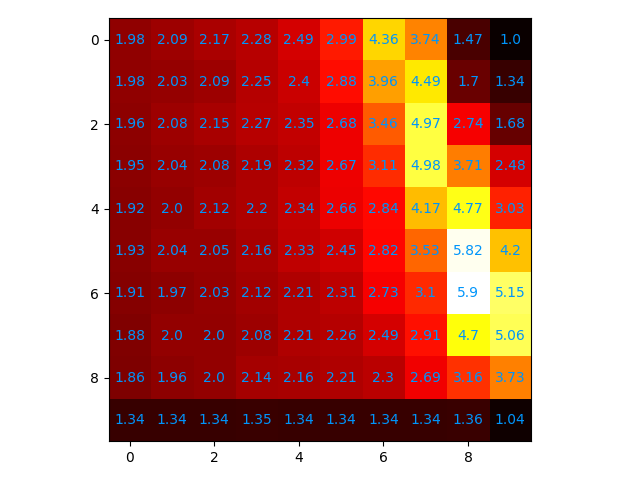
\includegraphics[width=8cm]{assets/msom_abcd}
    \caption{MSOM results}
\end{figure}


\begin{table}[h!]
    \centering
    \begin{tabular}{|c|c|} 
     \hline
     Parameter & Hodnota \\ 
     \hline\hline
     1 & 6  \\ 
     \hline
     2 & 7   \\
     \hline
     3 & 545  \\
     \hline
     4 & 545  \\
     \hline
     5 & 88 \\  
     \hline
    \end{tabular}
    \caption{Parametre leaky mSOM siete}
    \label{table:2}
\end{table}

\begin{figure}[H]
    \centering
    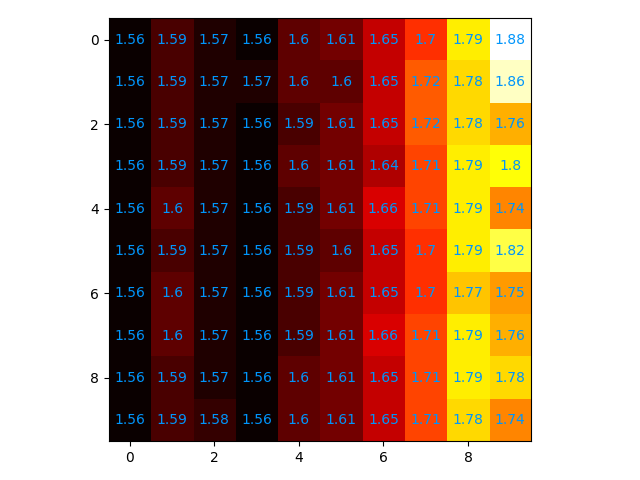
\includegraphics[width=8cm]{assets/leakymsom_abcd}
    \caption{Leaky MSOM results}
\end{figure}


\section{Experiment so SRN a Reberovým automatom}



